\documentclass{beamer}
\usepackage{graphicx}
\usepackage{listings}
\usepackage{xcolor}
\usepackage{tikz}
\usetheme{Madrid}
\usecolortheme{whale}

% Remove navigation symbols
\setbeamertemplate{navigation symbols}{}

% Custom footer
\setbeamertemplate{footline}{
  \begin{beamercolorbox}[wd=\paperwidth,ht=2.5ex,dp=1.125ex,leftskip=.3cm,rightskip=.3cm]{palette primary}
    \usebeamerfont{section in head/foot}
    \insertshorttitle\hfill\insertframenumber/\inserttotalframenumber
  \end{beamercolorbox}
}

% Title information
\title{Blockchain-Based Voting System}
\subtitle{A Secure and Transparent Voting Platform}
\author{Presented by: Your Name \\ Your Roll Number}
\institute{Department of Computer Science and Engineering\\
Your University Name}
\date{2024-2025}

\begin{document}

% Title slide
\begin{frame}
  \titlepage
  \begin{center}
    \vspace{0.5cm}
    \small{Guided by: Your Guide's Name}
  \end{center}
\end{frame}

\section{Introduction}
\begin{frame}{Introduction}
  \begin{itemize}
    \item Traditional voting systems face challenges in transparency and security
    \item Blockchain technology offers a decentralized solution for secure voting
    \item Smart contracts ensure automated and tamper-proof vote counting
    \item Ethereum platform provides robust infrastructure for implementation
  \end{itemize}
\end{frame}

\section{Problem Statement}
\begin{frame}{Problem Statement}
  \begin{itemize}
    \item Centralized voting systems are vulnerable to:
      \begin{itemize}
        \item Single point of failure
        \item Data manipulation
        \item Lack of transparency
        \item High operational costs
      \end{itemize}
    \item Need for a secure, transparent, and efficient voting mechanism
    \item Requirement for real-time vote verification and counting
  \end{itemize}
\end{frame}

\section{Applications}
\begin{frame}{Applications}
  \begin{itemize}
    \item Government Elections
      \begin{itemize}
        \item National and local elections
        \item Referendums
        \item Policy voting
      \end{itemize}
    \item Organizational Voting
      \begin{itemize}
        \item Board elections
        \item Shareholder voting
        \item Employee surveys
      \end{itemize}
    \item Educational Institutions
      \begin{itemize}
        \item Student council elections
        \item Faculty voting
        \item Course evaluations
      \end{itemize}
  \end{itemize}
\end{frame}

\section{Proposed Solution}
\begin{frame}{Proposed Solution}
  \begin{itemize}
    \item Blockchain-based voting system using:
      \begin{itemize}
        \item Ethereum smart contracts
        \item MetaMask for wallet integration
        \item Ganache for local development
        \item Hardhat for testing and deployment
      \end{itemize}
    \item Key Features:
      \begin{itemize}
        \item Decentralized architecture
        \item Real-time vote counting
        \item Transparent results
        \item Secure authentication
      \end{itemize}
  \end{itemize}
\end{frame}

\section{System Architecture}
\begin{frame}{System Architecture}
  \begin{center}
    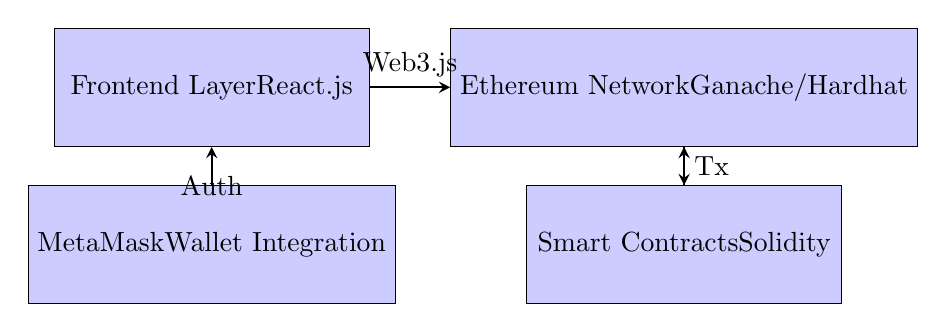
\begin{tikzpicture}[node distance=2cm]
      \tikzstyle{component} = [rectangle, minimum width=4cm, minimum height=1.5cm, text centered, draw=black, fill=blue!20]
      \tikzstyle{arrow} = [thick,->,>=stealth]
      
      \node (frontend) [component] {Frontend Layer\\React.js};
      \node (blockchain) [component, right of=frontend, xshift=4cm] {Ethereum Network\\Ganache/Hardhat};
      \node (contract) [component, below of=blockchain] {Smart Contracts\\Solidity};
      \node (wallet) [component, below of=frontend] {MetaMask\\Wallet Integration};
      
      \draw [arrow] (frontend) -- node[above] {Web3.js} (blockchain);
      \draw [arrow] (wallet) -- node[below] {Auth} (frontend);
      \draw [arrow] (blockchain) -- (contract);
      \draw [arrow] (contract) -- node[right] {Tx} (blockchain);
    \end{tikzpicture}
  \end{center}
\end{frame}

\section{Key Technologies}
\begin{frame}{Key Technologies}
  \begin{columns}
    \column{0.5\textwidth}
    \begin{itemize}
      \item \textbf{Ethereum}
        \begin{itemize}
          \item Decentralized platform
          \item Smart contract execution
          \item EVM compatibility
        \end{itemize}
      \item \textbf{Smart Contracts}
        \begin{itemize}
          \item Automated voting rules
          \item Immutable logic
          \item Gas optimization
        \end{itemize}
    \end{itemize}
    \column{0.5\textwidth}
    \begin{itemize}
      \item \textbf{Development Tools}
        \begin{itemize}
          \item Ganache (local blockchain)
          \item Hardhat (development environment)
          \item MetaMask (wallet)
        \end{itemize}
      \item \textbf{Frontend}
        \begin{itemize}
          \item React.js
          \item Web3.js
          \item Ethers.js
        \end{itemize}
    \end{itemize}
  \end{columns}
\end{frame}

\section{Algorithms and Techniques}
\begin{frame}{Algorithms and Techniques}
  \begin{itemize}
    \item \textbf{Smart Contract Algorithms}
      \begin{itemize}
        \item Candidate registration
        \item Voter authentication
        \item Vote casting
        \item Result calculation
      \end{itemize}
    \item \textbf{Security Measures}
      \begin{itemize}
        \item Cryptographic verification
        \item Role-based access
        \item Time-based restrictions
        \item Gas optimization
      \end{itemize}
  \end{itemize}
\end{frame}

\section{Results}
\begin{frame}{Results}
  \begin{columns}
    \column{0.5\textwidth}
    \begin{itemize}
      \item \textbf{Success Metrics}
        \begin{itemize}
          \item Secure vote casting
          \item Real-time counting
          \item Transparent results
          \item Low gas costs
        \end{itemize}
    \end{itemize}
    \column{0.5\textwidth}
    \begin{itemize}
      \item \textbf{Performance}
        \begin{itemize}
          \item Fast transaction processing
          \item Efficient gas usage
          \item Scalable architecture
          \item User-friendly interface
        \end{itemize}
    \end{itemize}
  \end{columns}
\end{frame}

\section{Conclusion}
\begin{frame}{Conclusion}
  \begin{itemize}
    \item Successfully implemented blockchain-based voting system
    \item Achieved key objectives:
      \begin{itemize}
        \item Decentralized architecture
        \item Secure voting process
        \item Transparent results
        \item User-friendly interface
      \end{itemize}
    \item Demonstrated practical application of blockchain technology
    \item Ready for real-world implementation
  \end{itemize}
\end{frame}

\section{Future Work}
\begin{frame}{Future Work}
  \begin{itemize}
    \item \textbf{Technical Improvements}
      \begin{itemize}
        \item Layer 2 scaling solutions
        \item Advanced encryption
        \item Mobile application
      \end{itemize}
    \item \textbf{Feature Enhancements}
      \begin{itemize}
        \item Multi-chain support
        \item Advanced analytics
        \item Automated auditing
      \end{itemize}
    \item \textbf{Deployment}
      \begin{itemize}
        \item Mainnet deployment
        \item Cross-platform support
        \item Global accessibility
      \end{itemize}
  \end{itemize}
\end{frame}

\section{References}
\begin{frame}{References}
  \begin{thebibliography}{9}
    \bibitem{ref1} Ethereum Foundation, ``Ethereum Documentation,'' 2024.
    \bibitem{ref2} MetaMask, ``MetaMask Documentation,'' 2024.
    \bibitem{ref3} Hardhat, ``Hardhat Documentation,'' 2024.
    \bibitem{ref4} Ganache, ``Ganache Documentation,'' 2024.
    \bibitem{ref5} Solidity, ``Solidity Documentation,'' 2024.
  \end{thebibliography}
\end{frame}

\begin{frame}
  \frametitle{}
  \begin{center}
    \begin{tikzpicture}[remember picture, overlay]
      \fill[blue!50] (current page.north west) rectangle (current page.south east);
      \node[anchor=center, font=\Huge\bfseries, text=white] at (current page.center){\Huge Thank You};
    \end{tikzpicture}
  \end{center}
\end{frame}

\end{document} 